\chapter{Background} \label{chapter:BACKGROUND}

This chapter describes prototype-based programming, the Lively Kernel, and CoExist.
These topics are relevant for this thesis as we present an approach for providing CoExist-like recovery support in prototype-based programming systems, which we implemented for the Lively Kernel system.

\section{Prototype-based Programming}

Prototype-based programming is object-oriented programming in which applications are constructed using objects, without requiring developers to define classes first.
Examples for genereal-purpose programming languages or systems that implement prototype-based programming are Self, JavaScript, and Kevo~\cite{Taivalsaari1992Kevo}.
In addition, many end-user programming systems, including Scratch~\cite{Maloney2010SPL}, Etoys~\cite{Kay2005Etoys}, Fabrik~\cite{Ingalls1988FVP}, and Lively Frabrik~\cite{Lincke2009LFW}, also enable users to express their programs through particular objects.

\paragraph{Similar Objects Without Classes}
Self and JavaScript incorporate prototypical inheritance.
They allow objects to inherit state and behavior directly from other objects through delegation: an object has a prototype to which it delegates when looking up a property in the object itself yields no results.
Kevo, in constrast, does not provide this kind of delegation, but instead allows to make full copies of objects, so objects in Kevo do not share behavior or state.
Programmers can create new objects with initially the same state and behavior as existing ones, but all objects remain self-contained.
That is, in Kevo, changing an object only changes that particular object and a particular object can only be changed by directly changing it, not by changing any other artifact.
To adapt many objects at once in Kevo, programmers can only use so-called \emph{module operations} that are evaluated on a group of objects. 

Despite this difference in whether properties can be shared among objects and how, thus, families of objects can be affected, prototype-based programming always allows to build programs from particular objects, in contrast to the class-based style of object-oriented programming, in which programs are expressed in more abstract definitions of structure and behavior.
In prototype-based programming, the parts of a program are objects with particular state, specific examples rather than general categories.

There are different advantages associated with this kind of programming:
\begin{itemize}
    \item \cite{Taivalsaari1996CVP} and \cite{Ungar1987SPS} argue that it might be easier for programmers to understand concrete examples than to grasp abstract classes. A concrete example provides particular values for its state and, in case of objects with a visual appearance, can be actually looked at.
    \item \cite{Ungar1987SPS} and \cite{Borning1986CVP} describe how prototype-based programming makes it easier to introduce one-of-a-kind objects with their own structure or behavior.
    \item \cite{Borning1986CVP} and \cite{Maloney1995Mor} make the point that especially editing visual objects can be more concrete with prototypes. Instead of writing code to define the appearance of objects, programmers can manipulate particular visual objects directly. Programmers could, for example, use the mouse to manipulate properties like the size, position, or to combine multiple basic elements into one composition. This way, programmers always see intermediate states and do not only receive feedback on explicit test runs in-between edit-compile-load cycles. 
\end{itemize}

\paragraph{Editing Objects At Runtime}
Many prototype-based programming systems, including all the examples given in this section, allow to manipulate objects at runtime.
Scratch, Etoys, Fabrik, Lively Fabrik, the Lively kernel, and Self also all provide tools to manipulate graphic objects and their behavior directly.
Such graphical objects range from basic objects like primitive shapes over interactive widgets to applications like presentation software or programming tools.
Programming at runtime, prototype-based programming, and direct manipulation of graphical objects seem properties that suit each other.


\section{The Lively Kernel}

The Lively Kernel is a browser-based programming system in the tradition of both Smalltalk and Self.
Development in the Lively Kernel happens at runtime.
The Lively Kernel incorporates tools and techniques to be completely self-sufficient.
Thus, programmers can create versions of the Lively Kernel with the Lively Kernel.

\subsubsection{Programming with Prototypes and Classes}

The Lively Kernel is based in the JavaScript programming language.
Therefore, the system and applications are expressed in a prototype-based object-oriented language that also provides prototypical inheritance.
At the same time, the Lively Kernel also provides a class system for JavaScript and considerable parts of the system itself are expressed using this class system.

One of the system parts expressed through classes is an implementation of Morphic~\cite{Maloney1995Mor}, a framework for developing graphical applications.
Programmers can alter graphical objects of this framework, which are called \emph{Morphs}, using direct manipulation and through a number of dedicated tools.

While Morphic framework itself is implemented using classes, morphs are an example of objects that are often edited directly and not through adapting existing or creating new classes.
Though each morph has a class, it can also have object-specific behavior.
Further, morphs can be created both through instantiating a Morphic class and through copying an existing morph.
The copy operation does not establish a prototypical inheritance relationship between the copy and the original, but instead copies the entire state, including of which class the copy is an instance of.
This way, the Lively Kernel mixes the class-based with the prototype-based style of object-oriented programming.

\subsubsection{Direct Manipulation of Morphs}

Programmers can change the position of morphs by dragging and the composition by an alternative dragging, which is called \emph{grabbing}.
That is, the composition of morphs is also part of Morphic and a morph can have submorphs.
This way, morphs are not limited to to be basic shapes or simple widgets, but can be entire user interfaces of arbitrary applications.
The Lively Kernel provides a set of manipulation tools, called \emph{Halos}, as shown in Figure~\ref{fig:Halos}, that developers can bring up directly at morphs.
The different halo buttons allow, for example, to resize~\textcircled{R}, rotate~\textcircled{T}, and copy~\textcircled{C} morphs.

\begin{figure}[h]
    \centering
    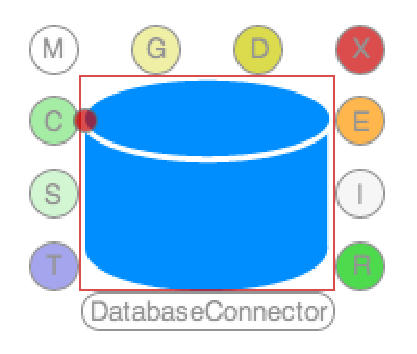
\includegraphics[width=0.3\textwidth]{figures/2_background/1_halos.pdf}
    \caption{The halo buttons of a basic morph.}
    \label{fig:Halos}
\end{figure}

Other halo buttons open specific tools, which are shown in Figure~\ref{fig:LivelyTools}, to further manipulate morphs:

\begin{figure}[h]
    \centering
    \includegraphics[width=\textwidth]{figures/2_background/2_LivelyTools.pdf}
    \caption{The Lively Kernel's tools to manipulate properties of morphs: the Inspector, the Style Editor, and the Object Editor.}
    \label{fig:LivelyTools}
\end{figure}

\begin{enumerate}
    \item The \emph{Inspector}~\textcircled{1} presents all the values that make up a morph's state. It also has a small code pane at the bottom, which is intended to be used to manipulate the state programmatically.
    \item The \emph{Style Editor}~\textcircled{2} allows to manipulate certain aspects of a morph's visual appearance. Programmers can use it to, for example, change a morphs color, border width, or the layout of its submorphs.
    \item The \emph{Object Editor}~\textcircled{3} is a tool dedicated to the object-specific behavior of morphs, which are called \emph{scripts} in the Lively Kernel. It shows all scripts of a particular morph, but also can add and adapt scripts.
\end{enumerate}


\subsubsection{Saving Morphs to the Shared Parts Bin Repository}

Another tool related to morphs is the Lively Kernel's \emph{Parts Bin}~\cite{Lincke2012LPC}, an object repository to commit and load specific versions of morphs.
Morphs saved to the Parts Bin are called \emph{parts} to emphasize the ability to reuse any of the morphic applications in the Parts Bin for other applications.
Figure~\ref{fig:PartsBin} shows the Parts Bin, opened on the \emph{Tools} category, which includes both the Style Editor and the Object Editor.
Both these tools are examples for graphical applications developed from available parts, with their logic expressed in scripts, and available to users through the Parts Bin.

\begin{figure}[h]
    \centering
    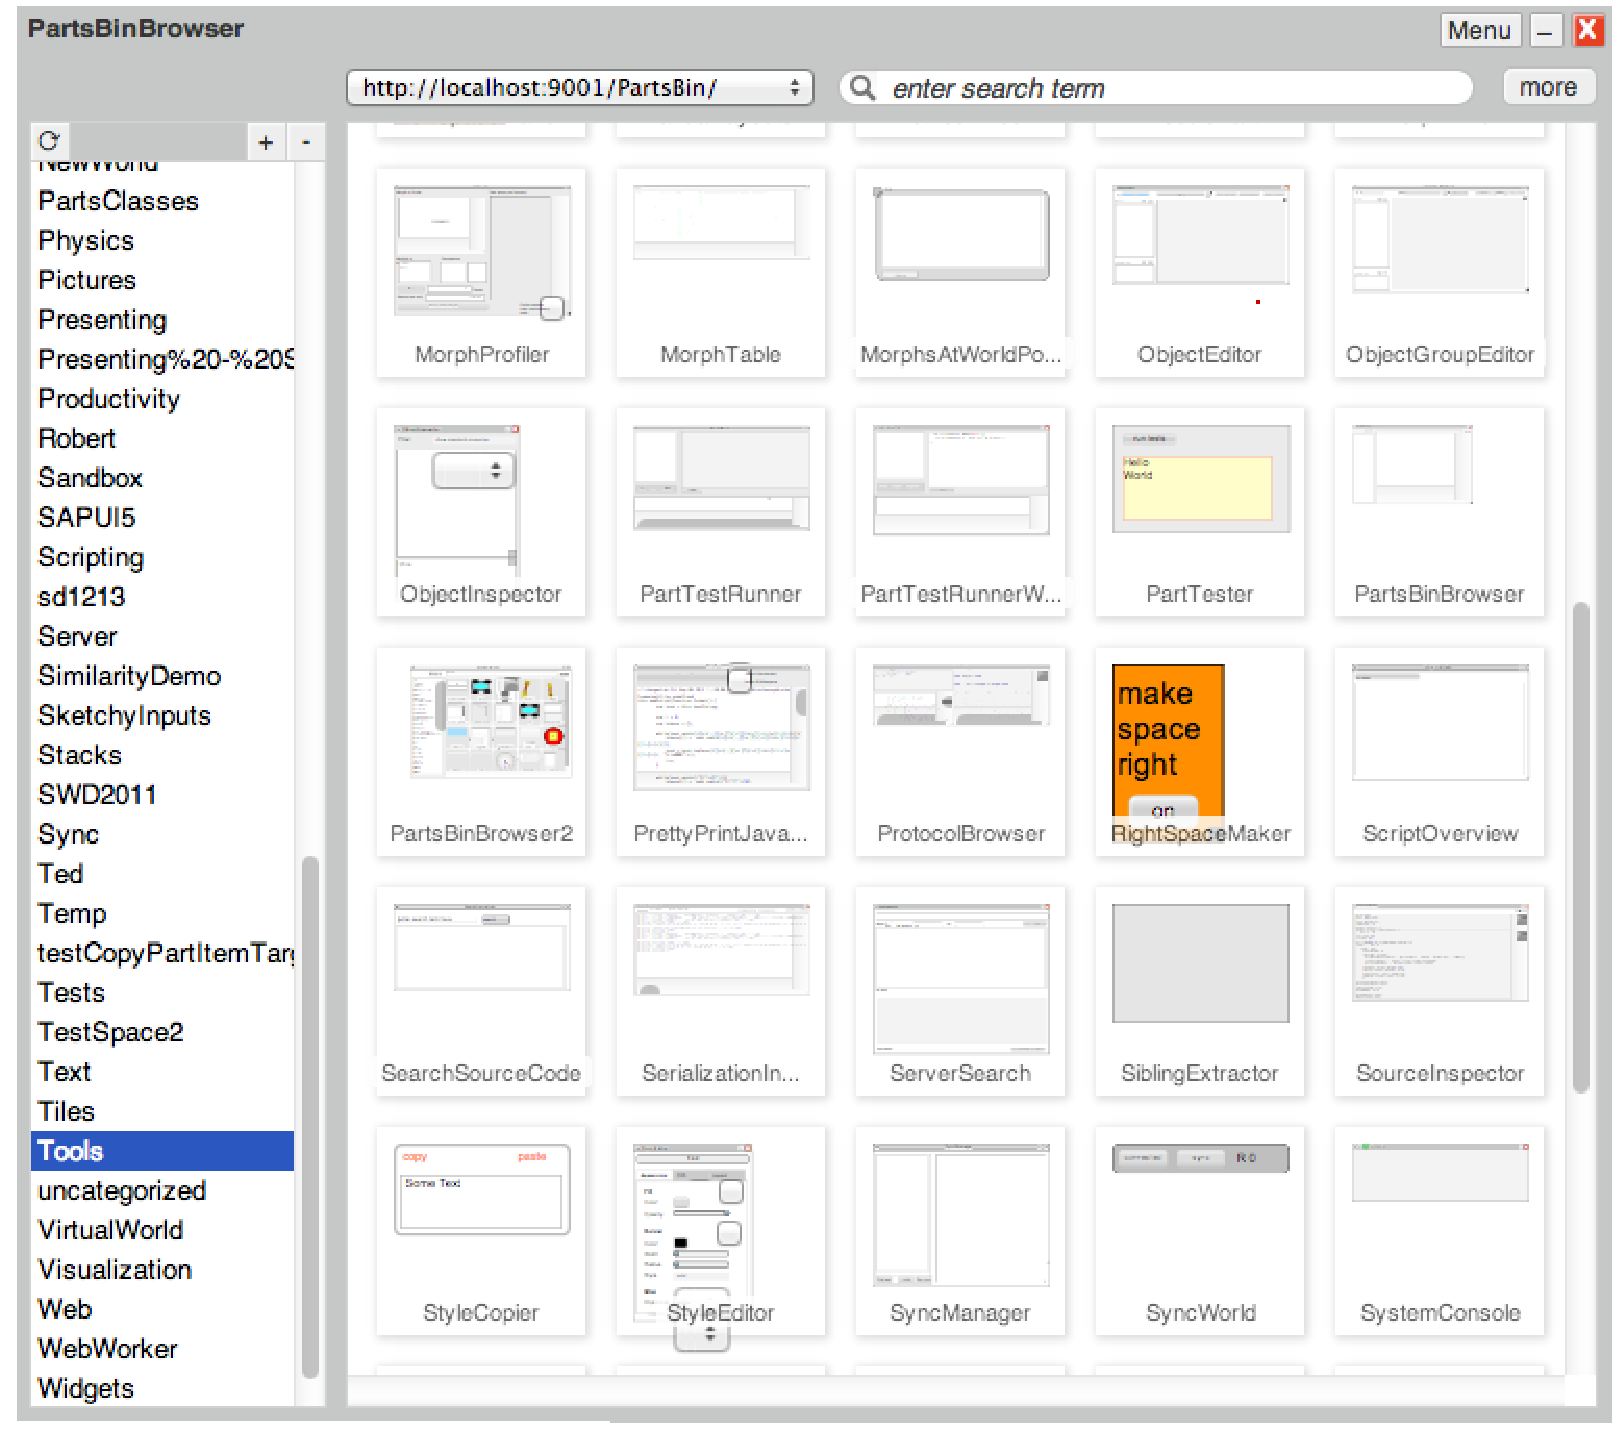
\includegraphics[width=0.7\textwidth]{figures/2_background/3_partsBin.pdf}
    \caption{The Lively Kernel's Parts Bin opened on the \emph{Tools} category.}
    \label{fig:PartsBin}
\end{figure}


The root of the scenegraph of visible morphs is called \emph{World}.
It is not shared via the Parts Bin, but can be saved as a Web page.
A world stores the state of all visible morphs when saved and that state can be reloaded with the world.
The Lively Kernel is always started with a world.

\section{CoExist}

CoExist\footnote{\url{http://www.bastiansteinert.org/coexist.html}, accessed February 28, 2014} supports programmers through automatic and continuous versioning.
CoExist preserves access to each indermediate development state with its respective source code and associated runtime information.
The states are recorded as separate version in their original order and along with change summaries, associated test results, and screenshots of the development environment.
Programmers can review their development sessions, inspect the impact each individual change had on test cases, and recover previous development states.
They can withdraw changes or only re-visit a previous state to recover partial information as, for example, the source code for a specific method.

\subsubsection{Tools to Recover Previous Development States}

CoExist provides two tools to help programmers benefit from the preserved development histories, shown in Figure~\ref{fig:CoExist}:

\begin{figure}[h]
    \centering
    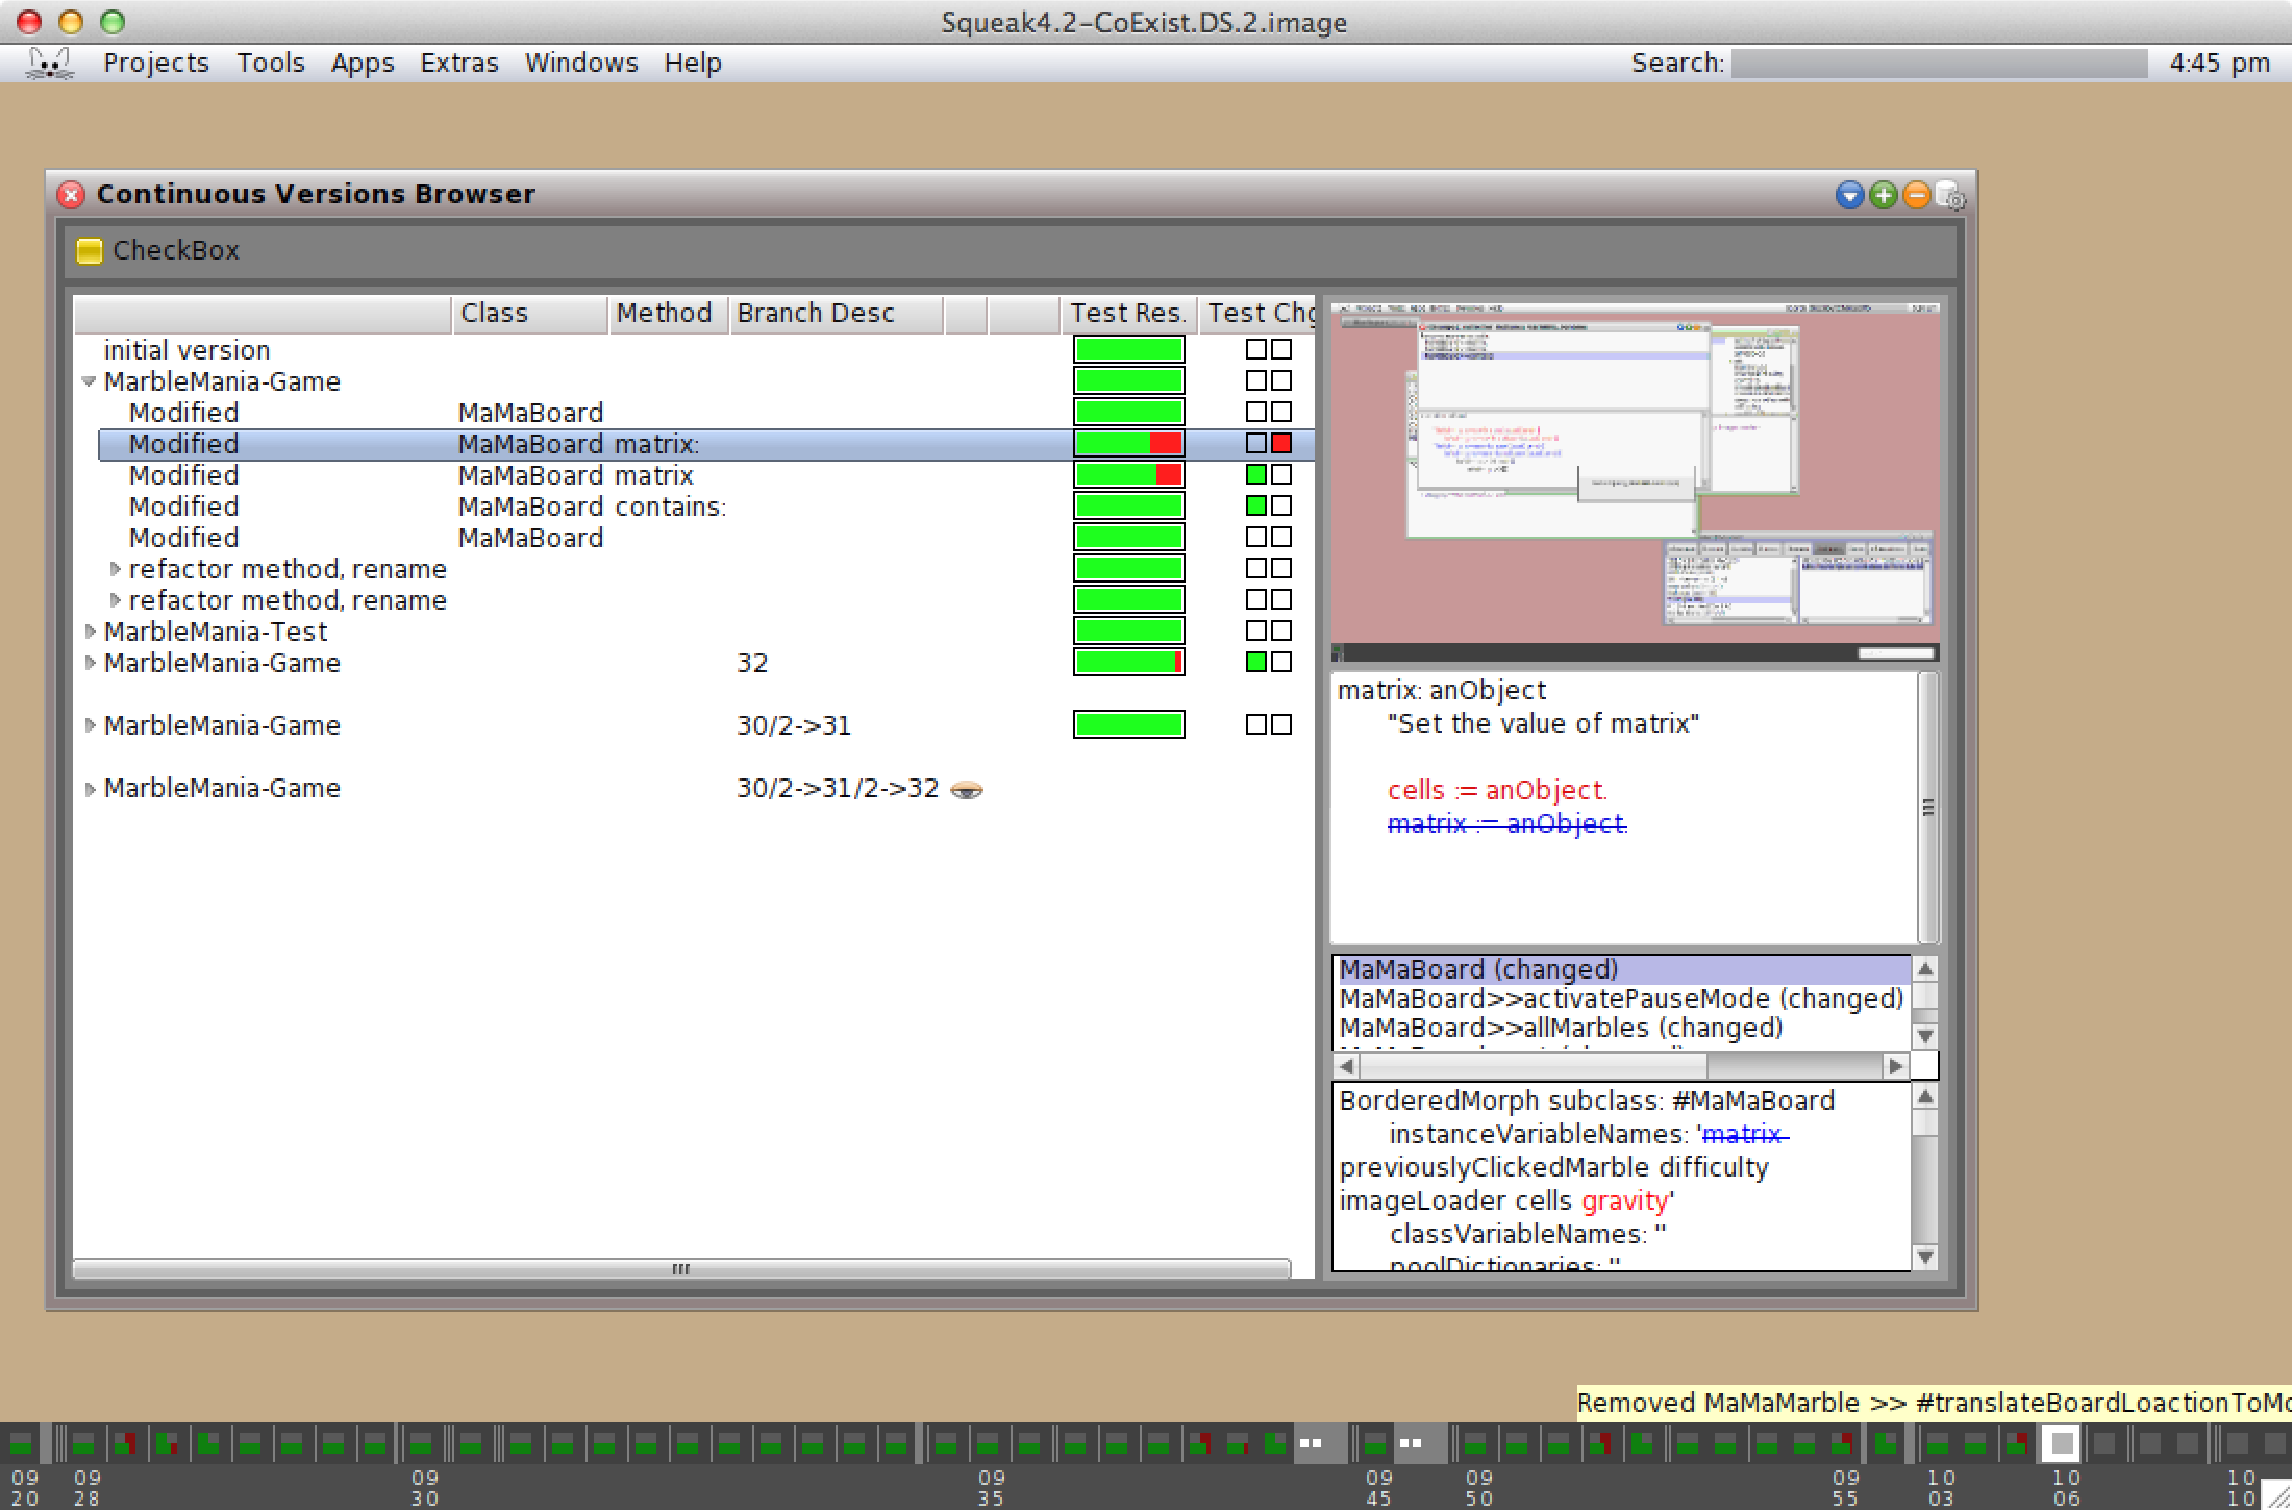
\includegraphics[width=\textwidth]{figures/2_background/4_coexistTools.pdf}
    \caption{CoExist's tools to manage the preserved development states: a timeline and a Version Browser.}
    \label{fig:CoExist}
\end{figure}

\paragraph{Timeline}
A \emph{timeline} tool at the bottom of the development environment presents each intermediate version through a small rectangle that indicates the impact on test cases: the bottom of the rectangle shows how many test cases passed and failed absolutely, while the top half highlights only test results affected by the changes of this particular version.
Hovering above such a version rectangle indicates what exactly changed in terms of methods and classes.
Clicking a version provides access to its source code and more information on test results, but also allows to re-establish the version.

\paragraph{Version Browser}
Besides the timeline of versions, a \emph{Version Browser} tool shows changes in a different layout and separately for different source code modules.
It presents the same information on test cases, but also offers diffs and how the development environment appeared visually in each version through screenshots.

\emph{In summary}, the tools support programmers in re-tracing their steps, understanding the impact of their actions, and in recovering information from previous development states.


\subsubsection{Benefits of Continuous Versioning}

CoExist is intented to reduce the effort that programmers usually put into recovery and, thereby, to encourage programmers to explore their ideas through actual development more often.

Without CoExist, either compensational or precautionary actions are necessary for recovery.
When programmers unintentionally introduce errors, decrease performance, or harm the program design, they can manually repair improperly changed code.
Alternatively, programmers can preserve specific versions to be able to easily withdraw changes later.
That is, they can reduce the cost of recovery by anticipating recovery needs beforehand.
Preserving versions manually is, however, also an effort and especially so when revision histories are expected to be well-documented and immediately useful.
For that, programmers need to assemble changes to meaningful increments, test these, and write helpful commit messages.
Testing each one directly is also advocated as it can help to find introduced problems directly intead of later analyzing long lists of changes that all could potentially have introduced a problem.

CoExist provides tool support for easy and fast recovery.
Developers do not have to take these explicit precautionary actions, but still are able to undo changes when necessary.
In this regard, CoExist is similar to undo/redo systems.
CoExist however provides access to the previous states of the entire system, not just particular source code views or files.
Further, it provides much more structure, as each version is associated with the static structure of the software system, is related to other versions in a timeline, and accompanied by test results.
Additionally, making changes to a previous state in CoExist does not overwrite the history, but creates a branch.

Instead of worrying about negative consequences when trying ideas, programmers can focus on their actual programming tasks and rely on CoExist to help in case any action unexpectedly needs to be undone.

